\documentclass[border=10pt]{standalone}

\usepackage{tikz}
\usepackage{tikzsymbols}
\usetikzlibrary{calc,patterns,shapes.geometric}

\def\centerarc[#1](#2)(#3:#4:#5){\draw[#1] ($(#2)+({#5*cos(#3)},{#5*sin(#3)})$) arc (#3:#4:#5);}

\begin{document}
	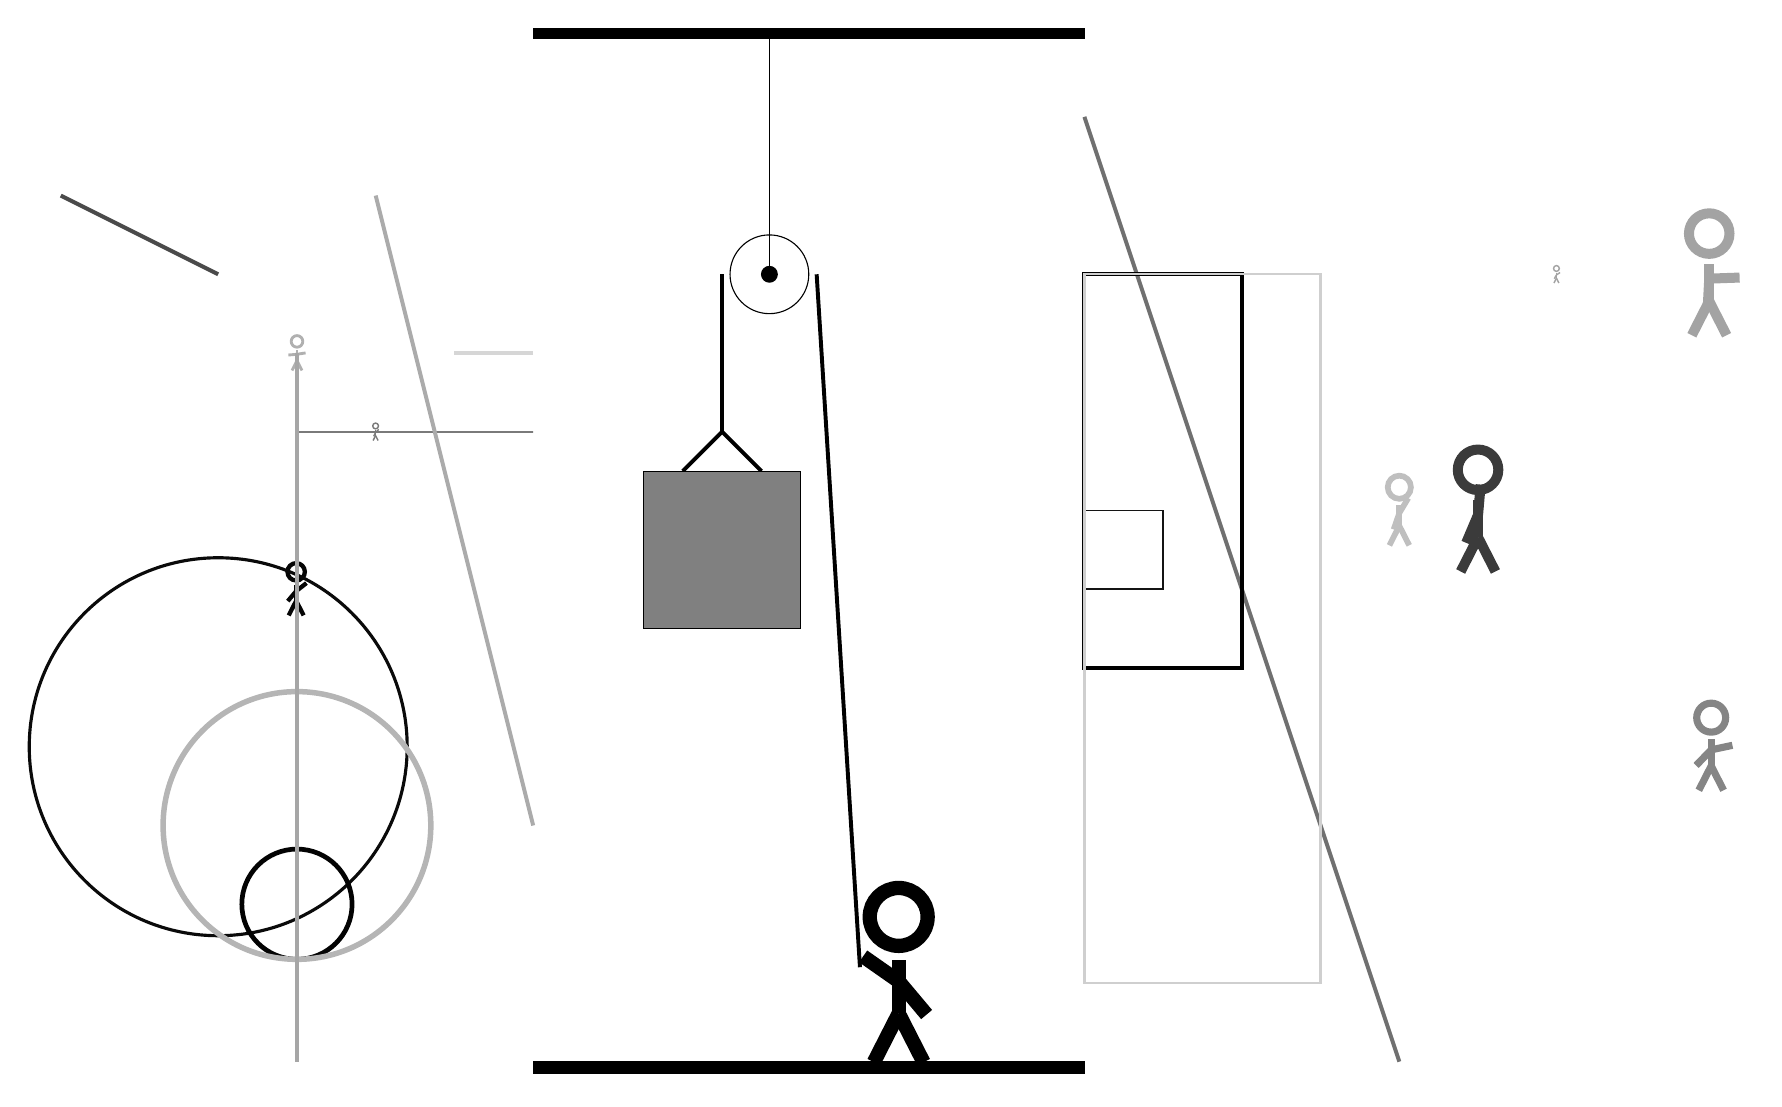
\begin{tikzpicture}
		%%%%% START %%%%%
		
		\draw[fill=black] (-2, 10) rectangle (5, 10.125);
		
		\draw (1, 7) circle (0.5);
		\draw[fill=black] (1, 7) circle (0.1);
		\draw (1, 10) -- (1, 7);
		
		\draw[line width=0.5mm] (-0.1, 4.5) -- (0.4, 5.0) -- (0.9, 4.5);
		\draw[fill=black!50] (-0.6, 4.5) rectangle (1.4, 2.5);
		
		\node[line width=0.2mm, color=black!31] at (-5, 6) {\Strichmaxerl[2][5][9]};
		
		\node[line width=0.4mm, color=black!98] at (-5, 3) {\Strichmaxerl[3][50][38]};
		\draw [line width=0.4mm, color=black!96](-6, 1) circle (2.4);
		\node[line width=0.6mm, color=black!25] at (9, 4) {\Strichmaxerl[4][71][59]};
		\draw[line width=0.5mm, color=black!71](-6, 7) -- (-8, 8);
		\draw[line width=0.5mm, color=black!56](5, 9) -- (9, -3);
		\draw[line width=0.5mm, color=black!100] (5, 2) rectangle (7, 7);
		
		\node[line width=0.5mm, color=black!52] at (-4, 5) {\Strichmaxerl[1][64][44]};
		\node[line width=0.5mm, color=black!48] at (13, 1) {\Strichmaxerl[5][46][12]};
		\node[line width=0.7mm, color=black!36] at (13, 7) {\Strichmaxerl[7][87][2]};
		\draw[line width=0.3mm, color=black!52] (-2, 5) rectangle (-5, 5);
		\draw [line width=0.6mm, color=black!99](-5, -1) circle (0.7);
		\draw[line width=0.2mm, color=black!92] (6, 3) rectangle (5, 4);
		
		\draw[line width=0.5mm, color=black!33](-2, 0) -- (-4, 8);
		\node[line width=0.3mm, color=black!77] at (10, 4) {\Strichmaxerl[7][67][85]};
		\node[line width=0.2mm, color=black!36] at (11, 7) {\Strichmaxerl[1][61][33]};
		
		\draw [line width=0.7mm, color=black!29](-5, 0) circle (1.7);
		\draw[line width=0.5mm, color=black!16](-2, 6) -- (-3, 6);
		\draw[line width=0.5mm, color=black!35](-5, 6) -- (-5, -3);
		\draw[line width=0.3mm, color=black!19] (5, -2) rectangle (8, 7);
		
		\draw[line width=0.5mm] (0.4, 7) -- (0.4, 5.0);
		\centerarc[line width=0.5mm](1, 7)(0:180:0.6);
		\draw[line width=0.5mm](1.6, 7) -- (2.15, -1.8);
		
		\node at (2.6, -1.9) {\Strichmaxerl[10][-35][-50]};
		
		\draw[fill=black] (-2, -3) rectangle (5, -3.15);
		
		%%%%% END %%%%%
	\end{tikzpicture}
\end{document}